\documentclass[../Head/Main.tex]{subfiles}
\begin{document}
\subsection{Lidar}
The implementation of the line and marble detection is done by designing a class called \texttt{lidar\_sensor} containing the key methods: \texttt{find\_marbles()}, \texttt{find\_lines()} and \texttt{merge\_lines()}. The first two key methods detect the marbles and lines in the image respectively. The third key method merges the lines on either side of a marble. The following two section describes the key methods in detail.
\subsubsection{Marble detection}
\label{subsubsec:Implementation_marble}
The marble detection method \texttt{find\_marbles()} processes the datapoints by checking if a point satisfies either one of the marble conditions. If so, it breaks and calculates the parameters described in section \ref{subsec:DesignMarbleDetection}.\par 
One marble condition is a threshold for the range between two point and is defined to 0.2. This condition ensures that a marble can be detected from points from a partial circle periphery. Another marble condition is a range, that ensures that a marble can be detected in outer edges of the lidar detection area. This range is defined as the subtraction of marble condition one from the sensor range for the lidar sensor.\par
To document the effectiveness of the marble detection, a series of tests was conducted.
\begin{figure}[H]
  \begin{subfigure}[b]{0.3\textwidth}
  	\centering
    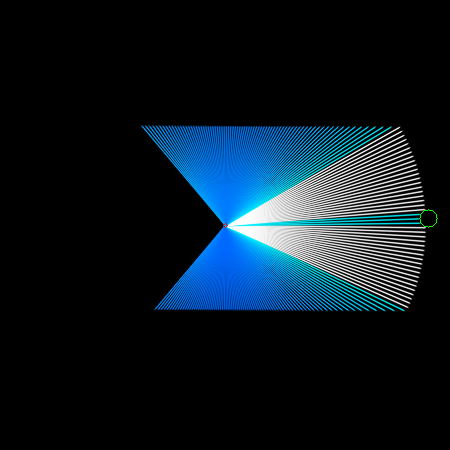
\includegraphics[width=1\textwidth]{Lidar/Test_2_marbles}
    \caption{Illustration of data for test 2}
    \label{fig:MarbleTest2}
  \end{subfigure}
  \hfill
  \begin{subfigure}[b]{0.3\textwidth}
  	\centering
    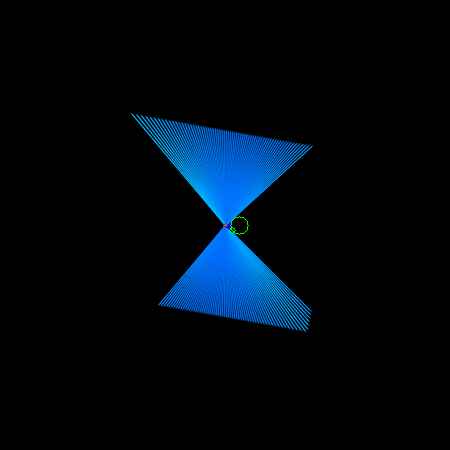
\includegraphics[width=1\textwidth]{Lidar/Test_3_marbles}
    \caption{Illustration of data for test 3}
    \label{fig:MarbleTest3}
  \end{subfigure}
  \hfill
  \begin{subfigure}[b]{0.3\textwidth}
    \centering
    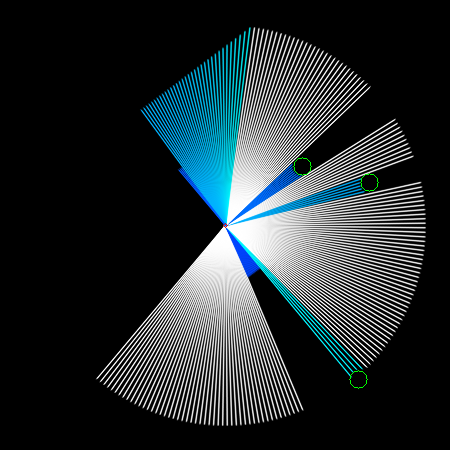
\includegraphics[width=1\textwidth]{Lidar/Test_5_marbles}
    \caption{Illustration of data for test 5}
    \label{fig:MarbleTest5}
  \end{subfigure}
  \caption{Illustration of data for marble detection tests}
\end{figure}
The marble detected on figure \ref{fig:MarbleTest2} verifies that the marble condition holds, and that a marble can be detected in the outer edge of the detection area. The same applies for one of the marbles on figure \ref{fig:MarbleTest5}. Figure \ref{fig:MarbleTest5} also shows that marbles can be detected anywhere in the sensor range. Sometimes the marble detection algorithm can detect an extra marble, where there is only one, as shown on figure \ref{fig:MarbleTest3}. 
\begin{figure}[H]
  \begin{subfigure}[b]{0.5\textwidth}
  	\centering
    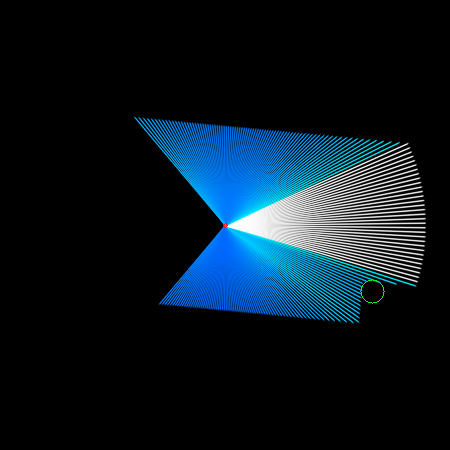
\includegraphics[width=0.6\textwidth]{Lidar/Test_6_marbles}
    \caption{Illustration of data for test 6}
    \label{fig:MarbleTest6}
  \end{subfigure}
  \hfill
  \begin{subfigure}[b]{0.5\textwidth}
  	\centering
    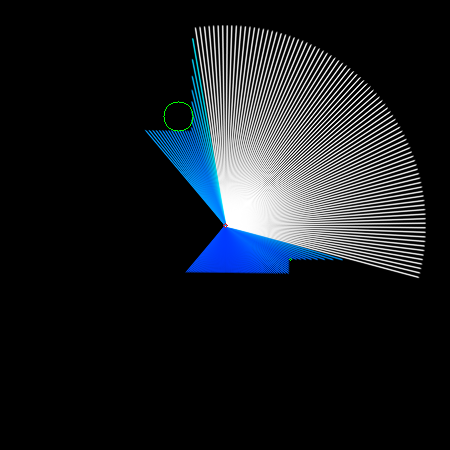
\includegraphics[width=0.6\textwidth]{Lidar/Test_7_marbles}
    \caption{Illustration of data for test 7}
    \label{fig:MarbleTest7}
  \end{subfigure}
  \caption{Illustration of data for marble detection tests}
\end{figure}
Figure \ref{fig:MarbleTest6} and \ref{fig:MarbleTest7} indicates that a marble can be detected in a corner, which might as well give problems. Due to the fact, that the robot will steer against marbles in the corners, the robot will hit an obstacle and tilt.\par
So, the marble detection algorithm performs as expected in some situations, but this also creates situations where the algorithm detects marbles, where there is none. 
\subsubsection{Line detection}
The line detection consists of the methods \texttt{find\_lines()} and \texttt{merge\_lines()}.\\
The method \texttt{find\_lines()} processes the datapoints by using the incremental line extraction algorithm. This algorithm first computes a line model for 2 points by calculating the line parameter described in section xx. When it recomputes the line model every time an extra point is added. Before recomputing the line model, the line parameters are stored. This means that the algorithm constantly updates the line parameters for the current and previous line model.\par
Due to the fact, that the algorithm constantly updates the line parameters for the current and previous line model, it does not have to recompute the previous line model, when the current line model does not satisfy the line conditions.
\begin{figure}[H]
  \begin{subfigure}[b]{0.3\textwidth}
  	\centering
    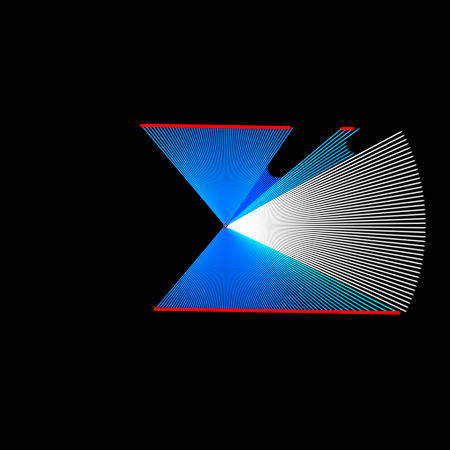
\includegraphics[width=1\textwidth]{Lidar/Test_1_lines}
    \caption{Illustration of data for test 1}
    \label{fig:LineTest1}
  \end{subfigure}
  \hfill
  \begin{subfigure}[b]{0.3\textwidth}
  	\centering
    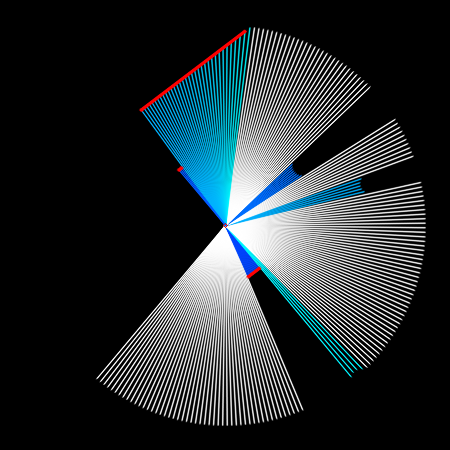
\includegraphics[width=1\textwidth]{Lidar/Test_5_lines}
    \caption{Illustration of data for test 5}
    \label{fig:LineTest5}
  \end{subfigure}
  \hfill
  \begin{subfigure}[b]{0.3\textwidth}
    \centering
    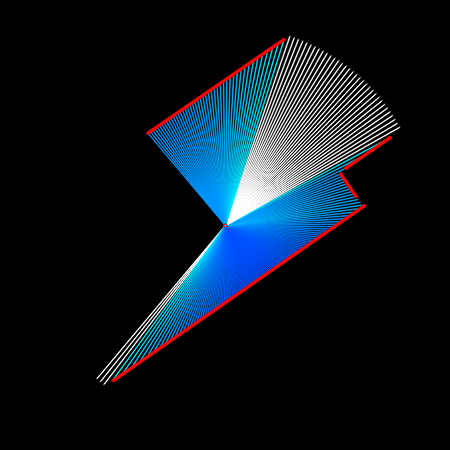
\includegraphics[width=1\textwidth]{Lidar/Test_6_lines}
    \caption{Illustration of data for test 6}
    \label{fig:LineTest6}
  \end{subfigure}
  \caption{Illustration of data for marble detection tests}
  \label{fig:LineTests}
\end{figure}
As mentioned in test {\color{red} missing reference}, the method \texttt{find\_lines} is reliable, since it find obstacles such as walls, corners and doorframes. This is also shown on figure \ref{fig:LineTests}.\par
All the found lines in the area of the sensor range is stored for further processing by the line merging method \texttt{merge\_lines()}.
The method \texttt{merge\_lines()} takes parameters from found lines, and check for two merging conditions The first condition is the angle between two found lines. This condition is called \texttt{threshold} and is defined to 0.1. The second condition is the area the marble provides shade. The algorithm does that by checking the difference in the angle from the end/start point of an found line to the closest line that strikes the marble. This condition is called \texttt{thresholdAlpha} and is defined to 0.5. The second condition prevents that two lines, that corresponds to doorframes, is merged. This means that the lines are not merged, if a marble is in front of a doorway to another room.\par
To document the effectiveness of the , a series of tests was conducted.
\begin{figure}[H]
  \begin{subfigure}[b]{0.5\textwidth}
  	\centering
    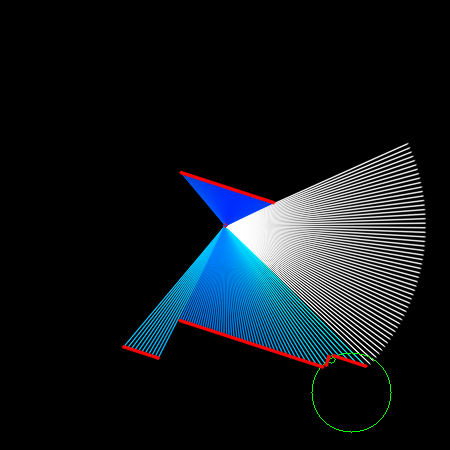
\includegraphics[width=0.6\textwidth]{Lidar/Test_7_lines}
    \caption{Illustration of data for test 7}
    \label{fig:LineTest7}
  \end{subfigure}
  \hfill
  \begin{subfigure}[b]{0.5\textwidth}
  	\centering
    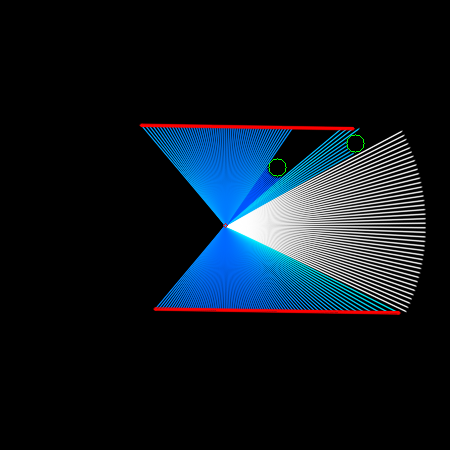
\includegraphics[width=0.6\textwidth]{Lidar/Test_8_lines}
    \caption{Illustration of data for test 8}
    \label{fig:LineTest8}
  \end{subfigure}
  \caption{Illustration of data for marble detection tests}
\end{figure}
The line merging method \texttt{merge\_lines()} is reliable is the sense that it is merging two lines, which is divided by a marble as shown on figure \ref{fig:LineTest8}. \par
The method depends on a marble detection method, which is not reliable, since it detects corners as marbles as shown on figure \ref{fig:LineTest7} and detects multiple marbles, when there is only one, as explained in section \ref{subsubsec:Implementation_marble}.
\end{document}